% vim:autoindent:set textwidth=78:

\section{Print Composer}\label{label_printcomposer}

% when the revision of a section has been finalized, 
% comment out the following line:
\updatedisclaimer

The print composer provides growing layout and printing
capabilities. It allows you to add elements such as the QGIS map canvas, 
legend, scalebar, images, and text labels. You can size, group 
and position each element and adjust the properties to create your layout. 
The result can be printed (also to Postscript and PDF), exported to image formats or to SVG.\footnote{Export to SVG supported, but it is not working 
properly with some recent QT4 versions. You should try and check individual 
on your system} See a list of tools in table~\ref{tab:printcomposer_tools}:

\begin{table}[h]\index{Print composer!tools}
\centering
\caption{Print Composer Tools}\label{tab:printcomposer_tools}\medskip
 \begin{tabular}{|l|p{6.9cm}|l|p{6.9cm}|}
 \hline \textbf{Icon} & \textbf{Purpose} & \textbf{Icon} &
 \textbf{Purpose} \\

 \hline 
\includegraphics[width=0.7cm]{mActionExportMapServer}
 & Export to an image format & 
 
\includegraphics[width=0.7cm]{mActionSaveAsSVG} & Export print composition 
 to SVG \\
 \hline 
\includegraphics[width=0.7cm]{mActionFilePrint} & Print or 
 export as PDF or Postscript &
 
\includegraphics[width=0.7cm]{mActionZoomFullExtent} & Zoom to
 full extend \\
 \hline 
\includegraphics[width=0.7cm]{mActionZoomIn} & Zoom in &
 
\includegraphics[width=0.7cm]{mActionZoomOut} & Zoom out \\
 \hline 
\includegraphics[width=0.7cm]{mActionDraw} & Refresh 
 view &
 
\includegraphics[width=0.7cm]{mActionAddRasterLayer} & Add 
 new map from QGIS map canvas \\
 \hline 
\includegraphics[width=0.7cm]{mActionSaveMapAsImage} & Add Image to 
 print composition &
 
\includegraphics[width=0.7cm]{mActionLabel} & Add label to print composition \\
 \hline 
\includegraphics[width=0.7cm]{mActionAddLegend} & Add new legend to 
 print composition & 
 
\includegraphics[width=0.7cm]{mActionScaleBar} & Add new scalebar to print
 composition\\
 \hline 
\includegraphics[width=0.7cm]{mActionSelectPan} & Select/Move item in 
 print composition &
 
\includegraphics[width=0.7cm]{mActionMoveItemContent} & Move content within
 an item \\
 \hline 
\includegraphics[width=0.7cm]{mActionGroupItems} & Group items of 
 print composition & 
 
\includegraphics[width=0.7cm]{mActionUngroupItems} & Ungroup items of print 
 composition \\
 \hline 
\includegraphics[width=0.7cm]{mActionRaiseItems} & Raise selected
 items in print composition &
 
\includegraphics[width=0.7cm]{mActionLowerItems} & Lower selected items 
 in print composition \\
 \hline 
\includegraphics[width=0.7cm]{mActionMoveItemsToTop} & Move selected
 items to top & 
 
\includegraphics[width=0.7cm]{mActionMoveItemsToBottom} & Move selected
 items to bottom \\
\hline
\end{tabular}
\end{table}

To access the print composer, click on the \toolbtntwo{mActionFilePrint}{Print}
button in the toolbar or choose \mainmenuopt{File} > \dropmenuopttwo{mActionFilePrint}{Print}.

\subsection{Using Print Composer}\label{label_useprintcomposer} 

Before you start to work with the print composer, you need to load some 
raster and vector layers in the QGIS map canvas and adapt their properties 
to suite your own convinience. After everything is rendered and symbolized to your liking you click the \toolbtntwo{mActionFilePrint}{Print} icon.

\begin{figure}[ht]
   \begin{center}
   \caption{Print Composer}\label{fig:print_composer_blank}\smallskip
   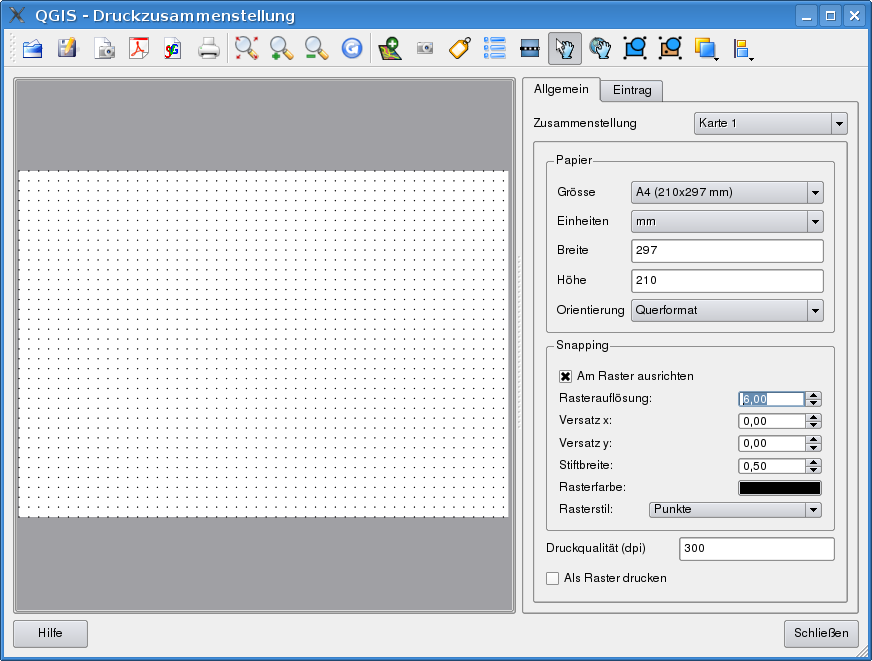
\includegraphics[clip=true, width=\textwidth]{print_composer_blank}
\end{center}  
\end{figure}

Opening the print composer provides you with a blank canvas to which you can 
add the current QGIS map canvas, legend, scalebar, images and text. Figure
\ref{fig:print_composer_blank} shows the initial view of the print composer before any elements are added. The print composer provides two tabs:

\begin{itemize}
\item The \tab{\textbf{General}} tab allows you to set paper size, orientation, and the print quality for the output file in dpi.
\item The \tab{\textbf{Item}} tab displays the properties for the selected map element. Click the \toolbtntwo{mActionSelectPan}{Select/Move item} 
icon to select an element (e.g. legend, scalebar or label) on the canvas. 
Then click the Item tab and customize the settings for the selected 
element.
\end{itemize}

You can add multiple elements to the composer. It is also possible to have 
more than one map view or legend or scalebar in the print composer canvas. 
Each element has its own properties and in the case of the map, its own 
extent.

\subsubsection{Adding a current QGIS map canvas to the Print Composer}

To add the QGIS map canvas, click on the \toolbtntwo{mActionAddRasterLayer}{Add new map from QGIS map canvas} button in the print composer toolbar and drag a 
rectangle on the composer canvas with the left mouse button to add the map. 
You will see an empty box with a \textit{"Map will be printed here"} message.
To display the current map, choose \selectstring{Preview}{Cache} in the map \tab{Item} tab.

You can resize the map later by clicking on the \toolbtntwo{mActionSelectPan}{Select/Move item} button, selecting the element, and dragging one of the blue handles in the corner of the map. With the 
map selected, you can now adapt more properties in the map \tab{Item} tab:

\begin{itemize}
\item Resize the map item specifying the width and height or the scale.
\item Define the map extend using Y and X min/max values or clicking the 
\button{set to map canvas extend} button.
\item Update the map preview and select, whether to see a preview from cache 
or an empty rectangle with a \textit{"Map will be printed here"} message. 
\item Define colors and outline width for the element frame, set a background color and opacity for the map canvas. You can also select or unselect to display an element frame with the \checkbox{frame} checkbox.
\end{itemize}


The map is now linked to the QGIS map canvas. If you change the view on the 
QGIS map canvas by zooming or panning or changing vector or raster properties, 
you can update the print composer view selecting the map element in the print composer and clicking the \button{Update Preview} button in the map 
\tab{Item} tab.

To move layers within the map element click on the map element in the 
canvas, click the \toolbtntwo{mActionMoveItemContent}{Move item content} icon 
and use the left mouse button to move the layers within the map element frame.

\begin{Tip}\caption{\textsc{Saving a print composer layout}}
\qgistip{If you want to save the current state of a print composer session, click on \mainmenuopt{File} > \dropmenuopttwo{mActionFileSaveAs}{Save Project As} to save the state of your workspace including the state of the current 
print composer session. It is planned but currently not possible to save print composer templates itself.
}
\end{Tip} 

\subsubsection{Adding other elements to the Print Composer} 

Beside adding a current QGIS map canvas it is also possible to add and customize legend, 
scalebar, images and label elements.

\minisec{Adding a legend}

To add a map legend, click the \toolbtntwo{mActionAddLegend}{Add new legend} icon and place 
the element with the left mouse button on the print composer canvas.

\minisec{Adding a scalebar}

To add a scalebar, click the \toolbtntwo{mActionScaleBar}{Add new scalebar} icon and place 
the element with the left mouse button on the print composer canvas.

\minisec{Adding a label}

To add a label, click the \toolbtntwo{mActionLabel}{Add label} icon and place the element 
with the left mouse button on the print composer canvas.

\minisec{Adding an image file}

To add any kind of image (e.g. logo or north arrow), click the 
\toolbtntwo{mActionSaveMapAsImage}{Add image} icon and place the element 
with the left mouse button on the print composer canvas.


Figure \ref{fig:print_composer_complete} shows the print composer after adding
each type of map element.
\begin{figure}[h]
   \begin{center}
   \caption{Print Composer with map view, legend, scalebar, and text added}
   \label{fig:print_composer_complete}\smallskip
   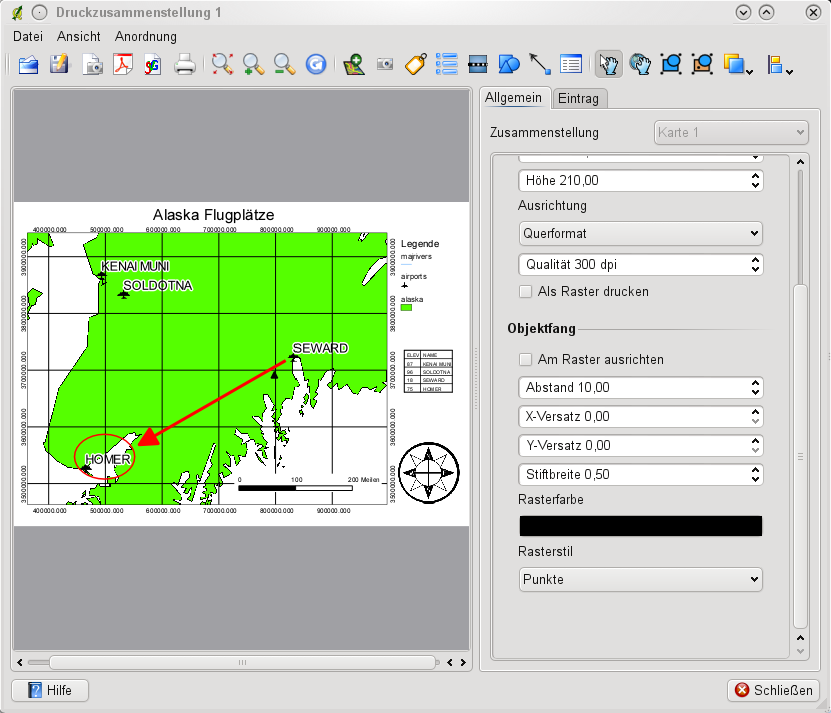
\includegraphics[clip=true, width=\textwidth]{print_composer_complete}
\end{center}  
\end{figure}

\subsubsection{Other Features}

The print composer has navigation tools to zoom in and out. To zoom in, click
the \button{Zoom in} tool. The print composer canvas will be scaled by a factor to 2. Use
the scrollbars to adjust the view to the area of interest. Zooming out works
in a similar fashion.

If you find the view in an inconsistent state, you can use the \button{Refresh} button
to redraw the print composer canvas.

\subsubsection{Creating Output}

The print composer allows you to print the layout to a printer, export to a PNG or
export to SVG. Each of these functions is available from the composer toolbar.

To save the composer canvas as a templates, click on the
%\toolbtntwo{composer_save_template}{Save Template As} 
button. Browse to the directory 
you like and save a template to use it again for another map canvas.

It is possible to export the result as an image by clicking on the
%FIXME \toolbtntwo{composer_export_image}{Export as image} 
button. 

To export the composer canvas as an  SVG (Scalable Vector Graphic), click on
the 
%FIXME \toolbtntwo{composer_export_svg}{Export as SVG} 
button. \textbf{Note:}
Currently the SVG output is very basic. This is not a QGIS problem, but a
problem of the underlaying Qt library. This will be sorted out in future versions.
 
